\documentclass[11pt]{article}

\usepackage{array}
\usepackage{parskip}
\usepackage{graphicx}
\usepackage{amsmath}
\usepackage{listings}

\usepackage[T1]{fontenc}
\usepackage{lmodern}
\usepackage[autostyle, english = american]{csquotes}
\MakeOuterQuote{"}

\newcolumntype{L}[1]{>{\arraybackslash}m{#1}}

\usepackage{pythonhighlight}

% Margins
\topmargin=-0.45in
\evensidemargin=0in
\oddsidemargin=0in
\textwidth=6.5in
\textheight=9.0in
\headsep=0.25in

\title{605.744: Information Retrieval \\ Programming Assignment \#3: Inverted Files}
\author{Sabbir Ahmed}
\date{\today}

\begin{document}
\maketitle	

\section{Introduction}
This paper describes the enhancements and features added to the Information Retrieval program started in Assignment 1 and upgraded in Assignment 2. Modifications include improvement in performance and adding support for batch processing and ranking queries.

% {'coronavirus': 1.9400969473898837, 'origin': 4.1451228967712135}

\section{Technical Background}
All of the source code is in Python 3.10. The program is split into several modules and follows an object oriented structure. The following is the directory structure of the source code:

% .
% ├── bin/
% ├── ir/
% │   ├── const.py
% │   ├── files.py
% │   ├── __init__.py
% │   ├── invertedfile.py
% │   ├── lexer.py
% │   ├── normalize.py
% │   ├── packer.py
% │   ├── retriever.py
% │   └── types.py
% ├── run.py
% ├── stats/
% └── tmp/

\begin{figure}[!ht]
    \centering
    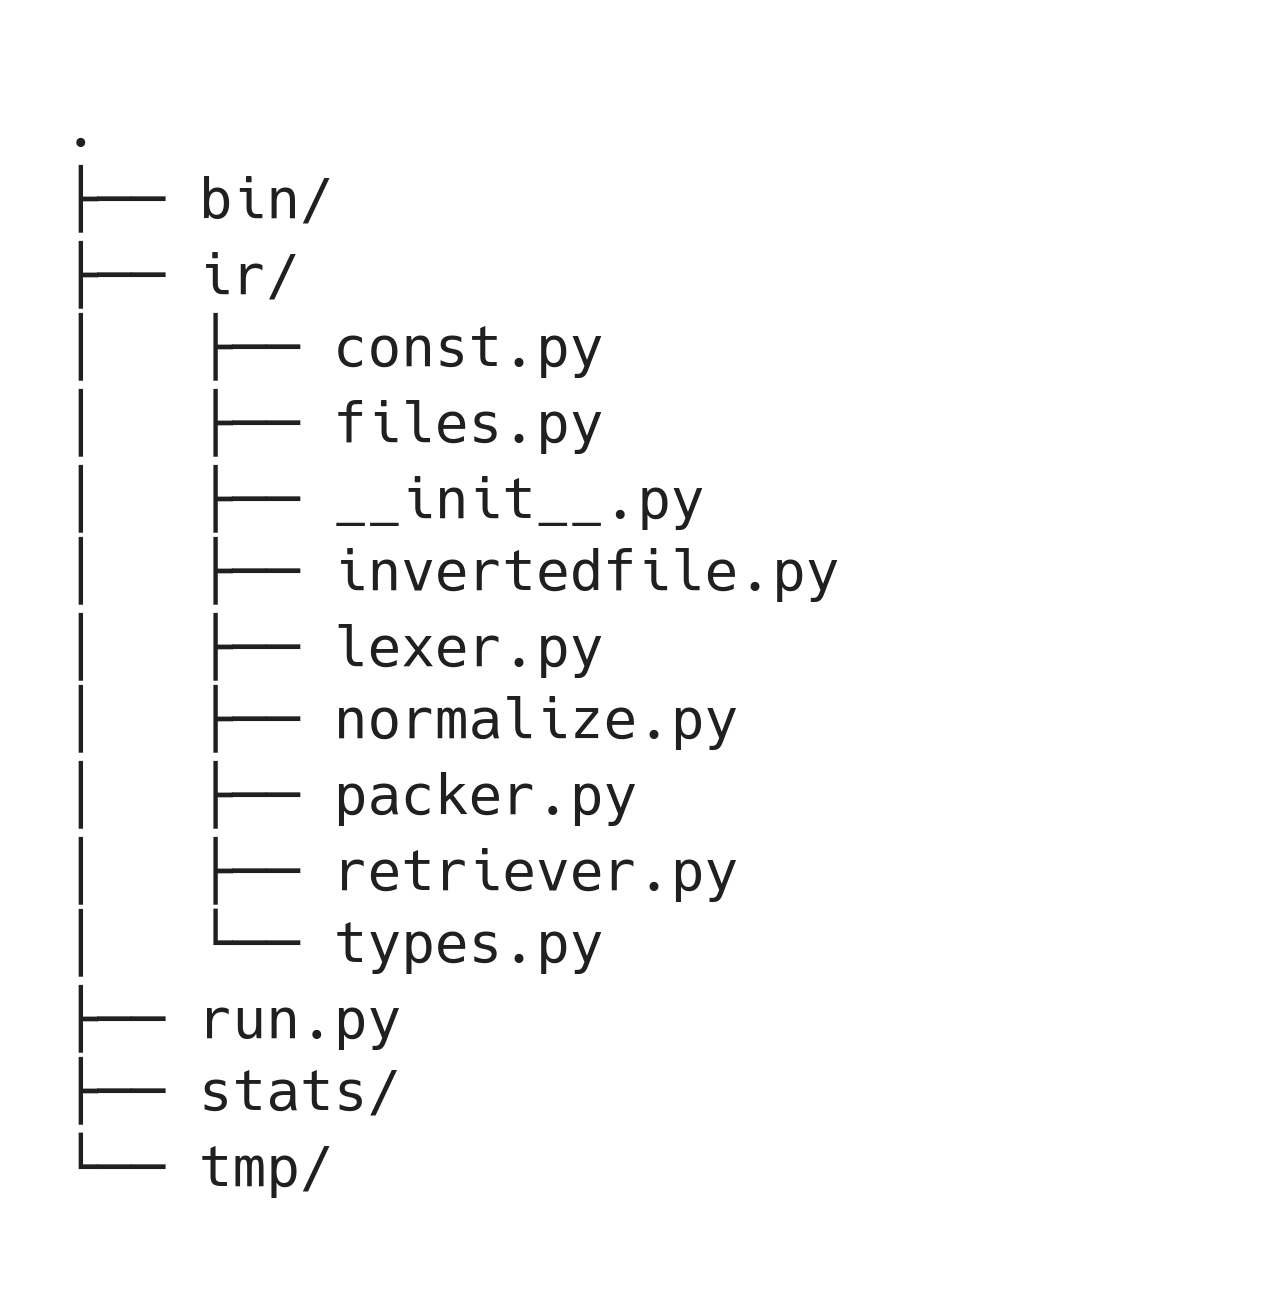
\includegraphics[scale=0.2]{statics/dirtree.png}
    \caption{Directory Hierarchy of Assignment 3}
\end{figure}

The source code for all of the files are attached in Appendix \ref{appendix:src}.

The total number of non-empty lines of code for the program totals to under 750.

\begin{figure}[!ht]
    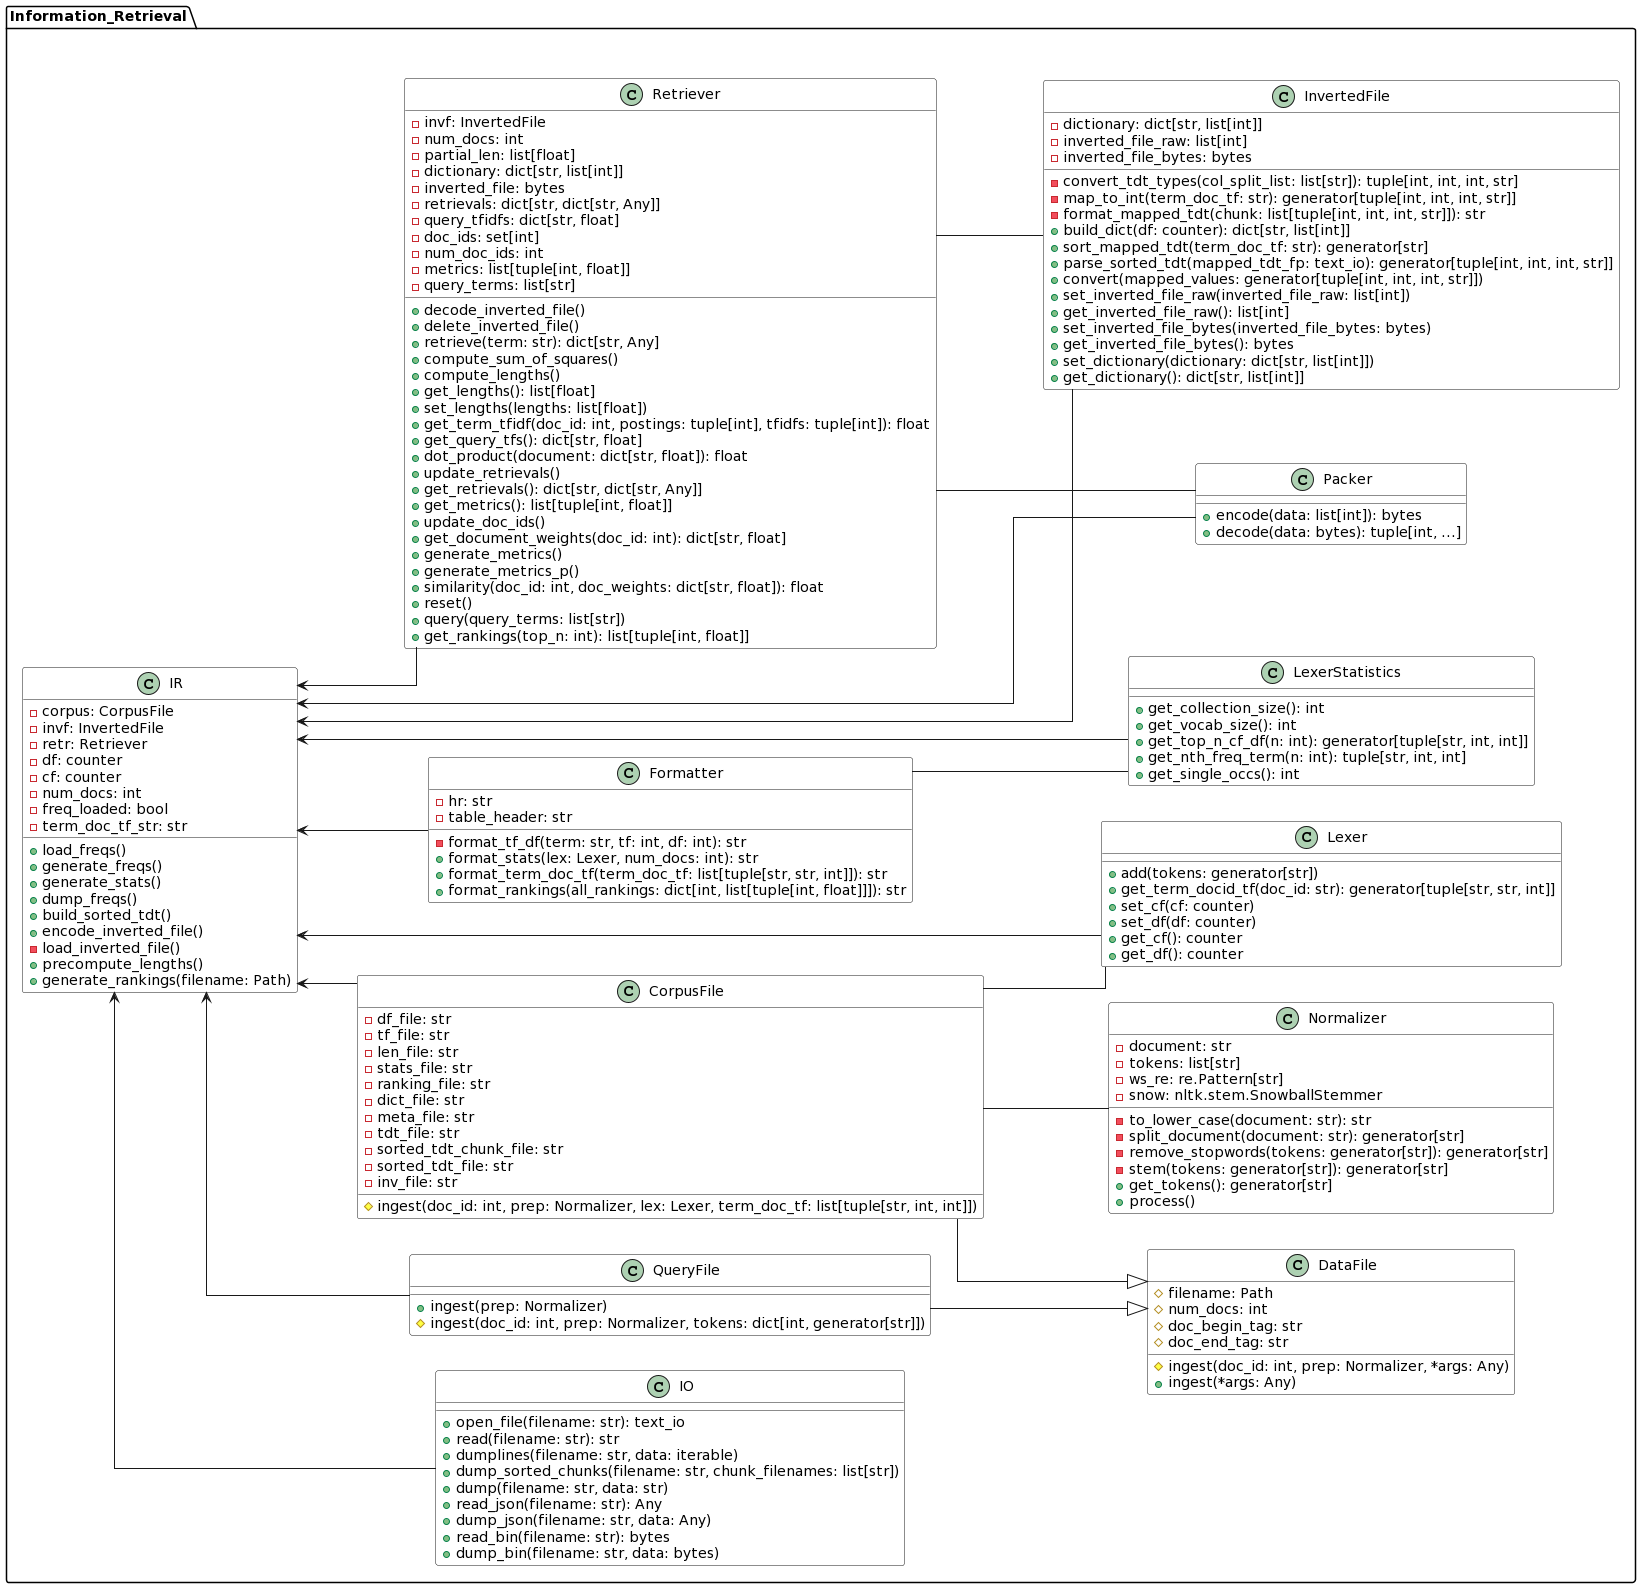
\includegraphics[scale=0.31]{statics/uml.png}
    \centering
    \caption{UML of Information Retrieval}
\end{figure}

\subsection{Existing Classes}

\subsubsection{Driver} \label{sec:driver}
The driver script for the program is \texttt{run.py}. The script uses command line options to process corpus files to perform the following operations:

\begin{enumerate}
    \item generate document and relative term frequencies
    \item generate statistics on corpus frequencies
    \item save frequencies to file
    \item extract term-docID-term frequency records and save to temporary files
    \item generate, encode and save inverted file
    \item compute document weights and save for repeated use
    \item process query files and generate rankings
\end{enumerate}

\subsubsection{\texttt{lexer.Lexer}}
The \texttt{Lexer} class had its methods on generating statistics separated into the \texttt{LexerStatistics} class.

\subsubsection{\texttt{files} Classes}
The \texttt{DataFile} class was renamed to \texttt{CorpusFile} and the \texttt{QueryFile} class was added to ingest query files. Both of these classes have been derived from the \texttt{DataFile} class.

The \texttt{Formatter} class has a new method to format rankings.

The \texttt{IO} class has a new method for writing chunks of data to files to be merged again. This method is only used for dumping chunks of sorted term-docID-term frequency records.

\subsubsection{\texttt{invertedfile.InvertedFile}}
The \texttt{InvertedFile} class received the following modifications:
\begin{itemize}
    \item the dictionary now only contains the term index, offset, length, and document frequency for each terms.
    \item the term-docID-term frequency records were sorted and saved to files in chunks. The chunk files are later merged to a single sorted file. This approach allows for the program to process  large corpuses without stressing the memory.
\end{itemize}

\subsection{\texttt{New Classes}}

\subsubsection{\texttt{retriever.Retriever}}
The\texttt{Retriever} class was added to compute document weights and rank queries.

The class precomputes document lengths to save to a file for repeated use. The document lengths are computed by reading the pre-generated inverted file and walking through each of the terms in the dictionary. The partial lengths of the documents are computed by adding the square of the TF-IDF of each of the term. The TF-IDF of a term is the product of its term frequency saved in the postings list of the inverted file and the logarithm of the inverse of its postings length. Once the entire inverted file is processed, the square root of each of the document partial lengths are computed and stored to file as the document vector lengths.

Once the document lengths have been computed, the class can process queries to compute similarities between its term weights against all of the documents in the corpus to generate rankings. The rankings are based on the cosine similarities between the query and the documents. The similarities are determined by evaluating the dot product of the query with each of the "relevant" documents and dividing the value with the product of their lengths. A document is considered "relevant" if it contains at least one of the query terms.

Generating this ranking is computationally expensive, even with the precomputed document lengths. The rankings of the query prompts were generated on a Debian-based Linux virtual machine with 2 cores, and generating the top 100 rankings for 50 queries per file may take hours to execute serially. Therefore, the class has been optimized to compute weights in parallel if the number of relevant documents exceed a threshold. The threshold value is assigned arbitrarily; 75,000 documents for \textit{cord19.topics.keyword.txt} and 90,000 documents for \textit{cord19.topics.questions.txt}.

\subsection{\texttt{Output Files}}
With the addition of several processes that rely on saving progress by writing no disk, the program makes use of numerous temporary files. The following table provides descriptions of each of the files:

\begin{table}[h]
    \begin{center}
        
        \begin{tabular}{| L{3.5cm} | L{12cm} |}
        \hline
        \textbf{File name} & \textbf{Description}
        \\ \hline
        corpus\_df.txt & Document frequencies of each normalized terms in the dictionary
        \\ \hline
        corpus\_cf.json & Relative term frequencies of each normalized terms in the dictionary
        \\ \hline
        corpus\_summary.txt & Summary statistics of the corpus as described in Assignment 1
        \\ \hline
        corpus\_len.json & Vector lengths of each of the documents in the corpus
        \\ \hline
        corpus\_rank.txt & Rankings generated from a query file sorted and formatted as described in the prompt
        \\ \hline
        corpus\_dict.json & Dictionary of the corpus containing each of the normalized terms mapping to their term index, inverted file offset, inverted file postings width, and their document frequency respectively
        \\ \hline
        corpus\_ndocs.txt & Number of documents in the corpus; this value is saved on disk to avoid having to reading large corpuses multiple times
        \\ \hline
        corpus\_tdt.txt & The term-docID-term frequency records saved to file after the entire corpus is processed
        \\ \hline
        corpus\_chunk\_$i$.txt ($i=0$ to $N$) & The sorted chunks of \texttt{corpus\_tdt.txt}; each of these  $N$ files are limited to \texttt{const.CHUNK\_SIZE} lines
        \\ \hline
        corpus\_sort.txt & The final sorted \texttt{corpus\_tdt.txt} file after merging all of its sorted chunks
        \\ \hline
        corpus\_if.bin & The inverted index file of the corpus
        \\ \hline
        \end{tabular}

    \end{center}
    \caption{Sizes of Files Computed Through the \texttt{stat} Command on a Debian Based Linux}

\end{table}



\section{Statistics and Observations}
\textit{cord19.topics.questions.txt}
In terms of the inverted files and dictionaries, the space they occupy on disk combined are significantly lower than the original document.

\begin{table}[h]
    \begin{center}
        
        \begin{tabular}{| l | r | l |}
        \hline
        \textbf{File} & \textbf{Size (in bytes)} & \textbf{Description} \\
        \hline
        headlines.txt & 39381610 & Input corpus file \\
        headlines\_dict.json & 4275427 & Generated dictionary JSON file \\
        headlines\_if.bin & 27774312 & Inverted binary file \\
        \hline
        \end{tabular}

    \end{center}
    \caption{Sizes of Files Computed Through the \texttt{stat} Command on a Debian Based Linux}

\end{table}

\section{Testing}
The tests described by the prompt were performed via the \texttt{test.py} driver script. The tokens to look up had to first be normalized through the \texttt{Normalizer} class.

\begin{lstlisting}[style=mypython,
    caption=Test 1: Document frequency and postings list for the terms: "Heidelberg"\, "cesium"\, "Trondheim"\, "crustacean"]
# NOTE: the normalization stems "crustacean" to "crustacea"
# and "crustaceans" to "crustacean"
tokens1 = normalize_test_terms(
    prep, ("Heidelberg", "cesium", "Trondheim", "crustaceans")
)
results1 = read_inverted_file(
    invf,
    tokens1,
    ("term", "postings", "postings_len"),
)
\end{lstlisting}

% \begin{figure}[!ht]
%     \centering
%     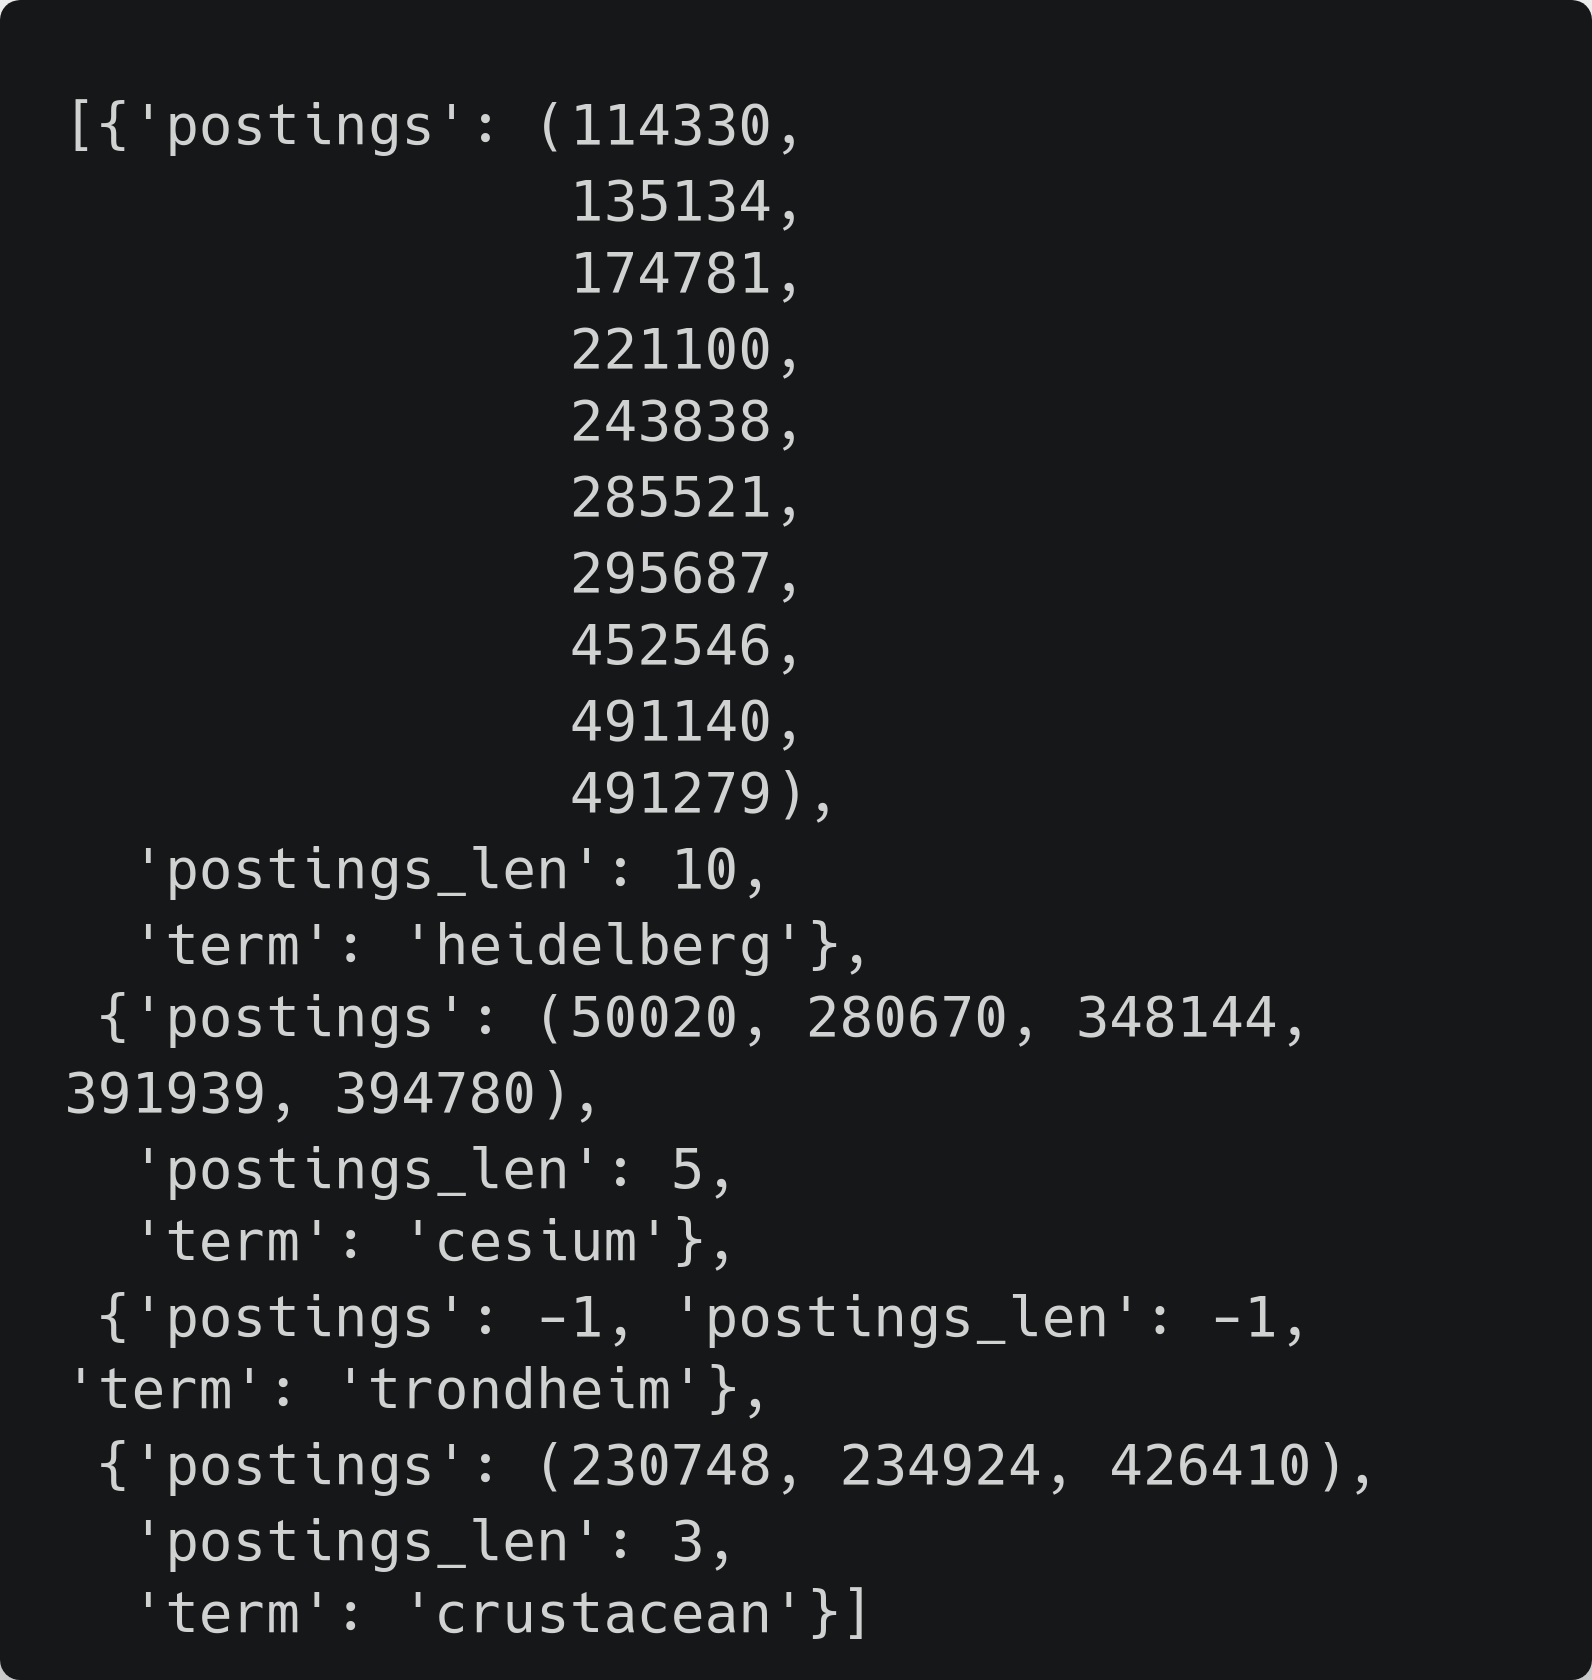
\includegraphics[scale=0.15]{statics/test1.png}
%     \caption{Output of Test 1}
% \end{figure}
% \clearpage
% \newpage

\begin{lstlisting}[style=mypython,caption=Test 2: Document frequency for the words: "Hopkins"\, "Stanford"\, "Brown"\, and "college"]
tokens2 = normalize_test_terms(
    prep, ("Hopkins", "Stanford", "Brown", "college")
)
results2 = read_inverted_file(invf, tokens2, ("term", "postings_len"))
\end{lstlisting}
% \clearpage
% \newpage

% \begin{figure}[!ht]
%     \centering
%     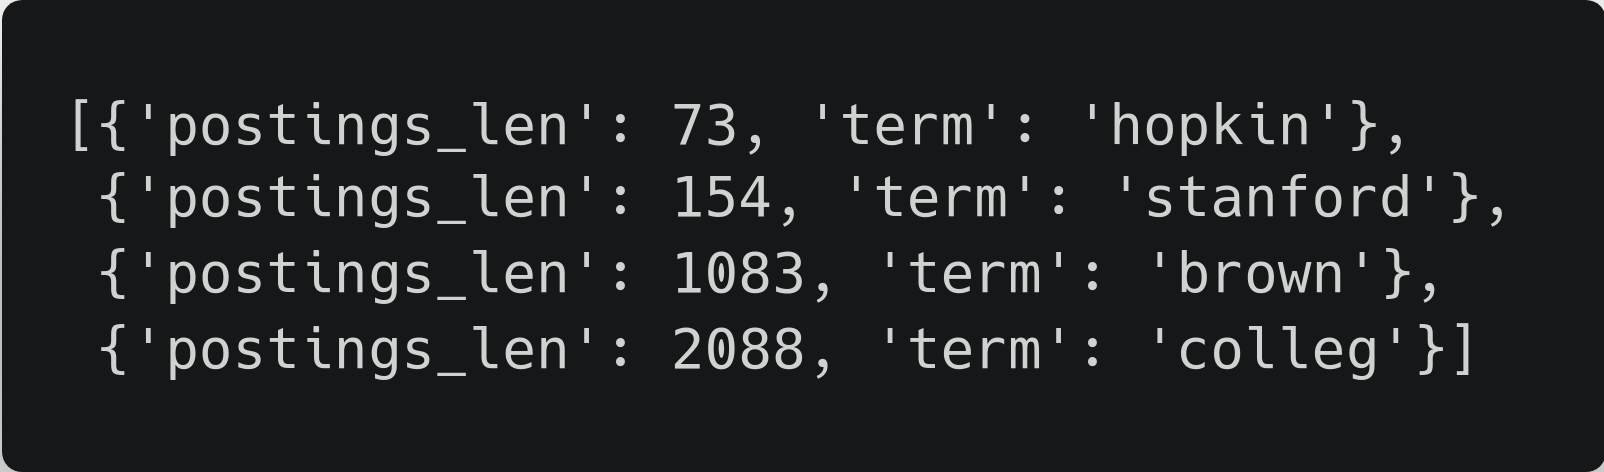
\includegraphics[scale=0.15]{statics/test2.png}
%     \caption{Output of Test 2}
% \end{figure}

\begin{lstlisting}[style=mypython,caption=Test 3: docids for documents that have both "Elon" and "Musk"]
# NOTE: the normalization stems "Musks" to "Musk"
tokens3 = normalize_test_terms(prep, ("Elon", "Musks"))
results3 = read_inverted_file(invf, tokens3, ("postings",))
elon, musk = results3
elon_postings, musk_postings = set(elon["postings"]), set(musk["postings"])
elon_musk_postings = elon_postings & musk_postings
\end{lstlisting}

% \begin{figure}[!ht]
%     \centering
%     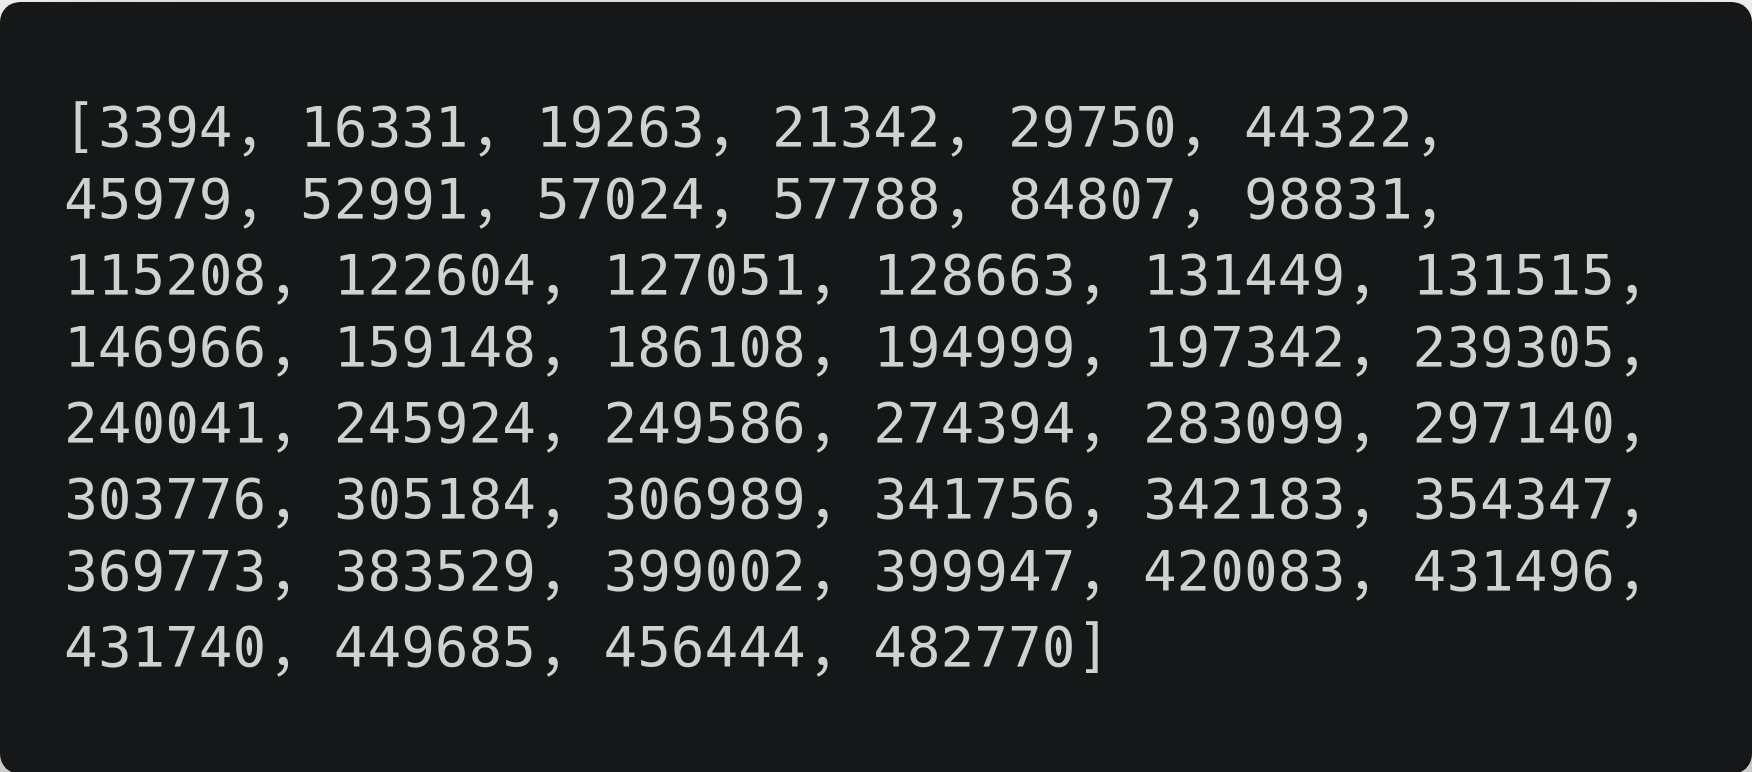
\includegraphics[scale=0.15]{statics/test3.png}
%     \caption{Output of Test 3}
% \end{figure}

\appendix

\section{Source Code} \label{appendix:src}

\inputpython{../ir/const.py}{../ir/const.py}
\inputpython{../ir/files.py}{../ir/files.py}
\inputpython{../ir/invertedfile.py}{../ir/invertedfile.py}
\inputpython{../ir/lexer.py}{../ir/lexer.py}
\inputpython{../ir/normalize.py}{../ir/normalize.py}
\inputpython{../ir/packer.py}{../ir/packer.py}
\inputpython{../ir/retriever.py}{../ir/retriever.py}
\inputpython{../ir/types.py}{../ir/types.py}

\inputpython{../run.py}{../run.py}

\section{Outputs} \label{appendix:outputs}

\lstinputlisting[caption=Statistics of 'cord19.txt',basicstyle=\small]{../outputs/stats/cord19_summary.txt}

\end{document}
